\documentclass[12pt]{article}
\usepackage{graphicx}

\pagestyle{empty}
\setcounter{secnumdepth}{2}

\topmargin=0cm
\oddsidemargin=0cm
\textheight=22.0cm
\textwidth=16cm
\parindent=0cm
\parskip=0.15cm
\topskip=0truecm
\raggedbottom
\abovedisplayskip=3mm
\belowdisplayskip=3mm
\abovedisplayshortskip=0mm
\belowdisplayshortskip=2mm
\normalbaselineskip=12pt
\normalbaselines

\begin{document}

\vspace*{0.5in}
\centerline{\bf\Large Design Document}

\vspace*{0.5in}
\centerline{\bf\Large Team 3}

\vspace*{0.5in}
\centerline{\bf\Large 11 March 2012}

\vspace*{1.5in}
\begin{table}[htbp]
\caption{Team}
\begin{center}
\begin{tabular}{|r | c|}
\hline
Name & ID Number \\
\hline\hline
John Alexander Landovskis & 9641394\\
Eric Regnier & 9332219\\
Rahmat Jaffari & 9095926\\
Bacacar Ndiaye & 9744258\\
Kam Shing Yip & 9602518\\
X & Y\\
X & Y\\
X & Y\\
X & Y\\
\hline
\end{tabular}
\end{center}
\end{table}

\clearpage

\section{Introduction}

The introduction of the document provides an overview of the entire document,
briefly introducing what are its goals, and what information is to be found in it.

\section{Architectural Design} \label{sec:arch}

This section must give a high-level description of the system in terms of its modules
and their respective purpose and exact interfaces.

\subsection{Architectural Diagram}
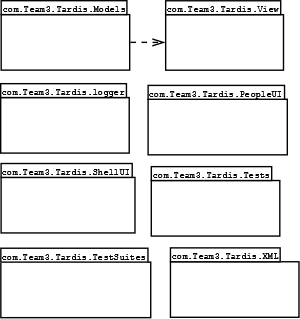
\includegraphics{diagrams/package_diagram}
\\
A UML class diagram or package diagram depicting the high-level structure of the system,
accompanied by a one-paragraph text describing the rationale of this design.
It is mandatory that the system be divided into at least two subsystems,
and that the purpose of each of these subsystems be exposed here.

\subsection{Subsystem Interface Specifications}

Specification of the software interfaces between the subsystems,
i.e. specific messages (or function calls) that are exchanged by the subsystems.
These are also often called ``Module Interface Specifications''.
Description of the parameters to be passed into these function calls in order to have a service fulfilled,
including valid and invalid ranges of values.
Each subsystem interface must be presented in a separate subsection.


\section{Detailed Design} \label{sec:detail}

Complete description of the system design, describing one subsystem separately in respective subsection.
UML class diagrams are to be used, as well as a short textual description describing the purpose of each class.

\subsection{Subsystem Models}

\subsubsection{Detailed Design Diagram}

UML class diagram depicting the internal structure of the subsystem,
accompanied by a paragraph of text describing the rationale of this design.

\subsubsection{Units Description}

List each class in this subsystem and write a short description of its purpose,
as well as notes or reminders useful for the programmers who will implement them.
List all attributes and functions of the class.

\section{Dynamic Design Scenarios}

\subsection{Add Scenario}
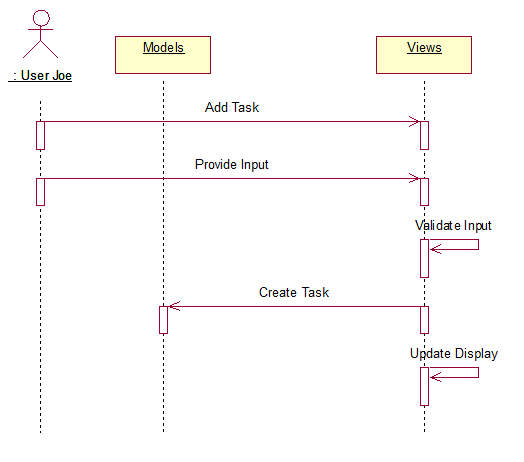
\includegraphics{diagrams/add_sequence_diagram.png}


\subsection{Delete Scenario}
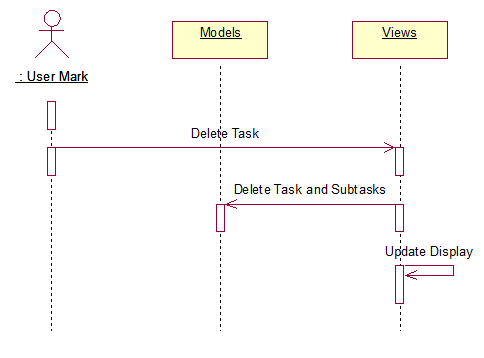
\includegraphics{diagrams/delete_sequence_diagram.png}



\end{document}
